\section{Scope, evidence, and the meaning of progress}\label{sec:scope}

The purpose of this retrospective is to explain what was built, which
questions were tested, what improved, what was corrected, and what remains
unresolved. Its organising question is the elliptic-curve discrete
logarithm problem (ECDLP): given a public point $G$ of order $r$ and
$Q=[d]G$, recover $d\bmod r$. The programme approaches this question from
several directions at once: faster generic solvers, non-generic relation
generation, algebraic systems, alternative representations and groups,
structural prediction, and reproducibility infrastructure.

The repositories contain enough work to require both a readable synthesis
and a searchable catalogue. This paper supplies the synthesis; the
accompanying CSV and JSON files supply the catalogue. It extends the
earlier fourteen-week index-calculus manuscript to April--October and to
the wider portfolio. The earlier manuscript is a useful guide, but its
figures and conclusions are re-read against their source studies and later
corrections rather than inherited wholesale.\src{PRIOR}

\subsection{Corpus and temporal boundary}

The review window is 19 April through 19 October 2026, UTC. The main
\texttt{crypto} repository was created on 25 April; consequently this
window contains its entire initial development. Snapshots were captured
independently on 19 October. They are not an atomic snapshot of all
machines, branches and external storage. The \texttt{cryptanalysis}
account default was an active development branch; the primary content
review deliberately pins \texttt{main} separately. This matters: its
\texttt{main} snapshot has 48,811 tracked entries, while the initially
observed default branch had 16,091.

\begin{longtable}{@{}p{3.5cm}r r p{3.1cm}@{}}
\toprule Repository & Entries & Window commits & Pinned commit \\
\midrule\endhead
WDSat & 89 & 2 & \texttt{cf146c780f2e} \\
autolab & 305 & 0 & \texttt{f1c783082328} \\
cairn & 920 & 537 & \texttt{6bb3a52c88f5} \\
cryptanalysis & 48,811 & 963 & \texttt{6e170e48882e} \\
crypto & 114,791 & 8,499 & \texttt{4f9ea9480b17} \\
crypto-autoresearcher & 138,314 & 22,794 & \texttt{d0f70c0a0905} \\
crypto-lean & 33 & 4 & \texttt{148f5dc389b3} \\
cryptologic-archives & 156 & 3 & \texttt{1096f83076a7} \\
ecbench & 9 & 1 & \texttt{5ca79764b725} \\
ecc-challenges & 433 & 101 & \texttt{4b4d47349b53} \\
ecdlp-cost-challenge & 79 & 49 & \texttt{2e215f1d503e} \\
ecdlp-prime-field-smallness & 66 & 5 & \texttt{4f20be9b36ff} \\
ecdsafail-challenge & 50 & 1,172 & \texttt{b6b648f4377f} \\
eigenx & 201 & 12 & \texttt{88f88a2da7bc} \\
ghs-trapdoor & 2 & 3 & \texttt{93981a150972} \\
isogeny-labs & 136 & 38 & \texttt{d613806737c7} \\
ml-cryptanalysis & 214 & 71 & \texttt{9c06ddee943c} \\
rho-blackwell & 320 & 18 & \texttt{5c3db3907924} \\
the-sqisign & 438 & 4 & \texttt{4c42deee64ee} \\
\bottomrule\end{longtable}


``Entries'' counts the tracked tree, not source lines, distinct programs,
or experiments. ``Window commits'' counts unique commits reachable from
that snapshot, filtered on committer time. It includes merge commits and
the history of imported or forked code. For example, the 1,172 window
commits reachable from the quantum-challenge fork cannot be credited as
1,172 contributions by this programme. Conversely, the Autolab snapshot's
zero window commits does not mean that no Autolab experiments occurred:
results and modified work are present in other branches and in the
autoresearcher migration records.

The three central histories contain 32,256 window commits: 8,499 in
\texttt{crypto}, 963 in \texttt{cryptanalysis/main}, and 22,794 in
\texttt{crypto-autoresearcher}. The portfolio's 34,276 snapshot-reachable
commits are distinct by commit hash across these nineteen snapshots.
Current branch metadata extends the union to 49,936 commits over 5,144
heads. Deleted branches, unreachable commits, uncommitted local work and
unavailable external artifacts remain outside that union. Branch content
is selectively reviewed; fetching its commit metadata is not a scientific
audit of every branch.

\begin{figure}[htbp]
\centering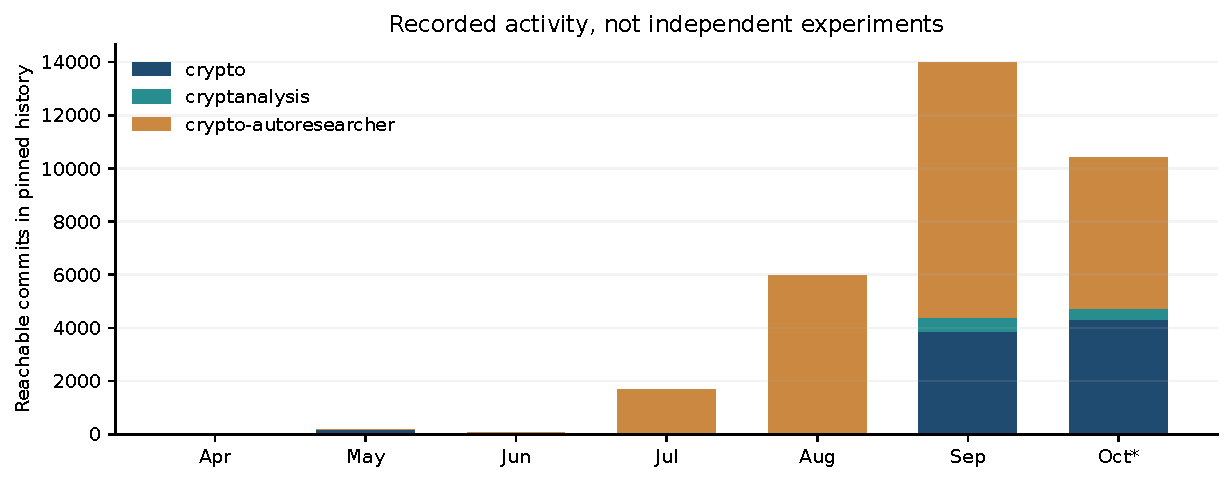
\includegraphics[width=\linewidth]{figures/activity.pdf}
\caption{Recorded activity in the three core pinned histories by
committer month. Merge and non-merge commits both occur in the histories.
Counts indicate archival volume, not independent experiments, researcher
hours, authorship, novelty or scientific success. October is partial.}
\label{fig:activity}
\end{figure}

\subsection{How the review was carried out}

The collection procedure used blobless Git histories, full tracked-tree
inventories, sparse content materialisation, repository indexes, ledger
parsing, and focused reads of studies and their code paths. The catalogue
contains 21,006 materialised Markdown documents under the documented size
and directory policy. A document's presence in that index means its title,
path and bytes were catalogued; it does not mean that every sentence was
manually assessed. A directory is similarly a navigational unit: several
directories can describe one study, while one directory can contain many
runs.

The 4,075 directory records cover \texttt{research/},
\texttt{experiments/}, \texttt{benchmarks/} and \texttt{papers/} across the
snapshots. The ledger catalogue parses 16,587 YAML files with a safe loader;
24 additional files could not be parsed by that loader and are retained
as explicit failures. Some root-level legacy records, archives and
checkpoints repeat or supersede other records. Record totals therefore
cannot be interpreted as distinct hypotheses or independent validations.
Both source paths and identifiers are retained so a reader can deduplicate
for a particular question.

The first synthesis used selective deep review. The subsequent request to
read everything prompted full-text reading of all fifteen root research
notes in the declared group, all twenty-one Markdown files in the pinned
ML tree, all nineteen ten-lead claim statements and all ten lead
descriptions. It also added complete reads of two implementation files and
two proof sources. These bounded completions do not complete the corpus.
The reading ledger records 94 fully read files (1,117,504 distinct bytes),
50 previously focused sources without complete reading receipts, and
305,223 entries without a reading receipt. Indexing, parsing and hashing
never count as reading. Appendix~\ref{app:reading} defines this boundary
and the unresolved exhaustive-reading obligation.

The review freshly checked byte hashes of all 19 frontier-session record
files, counted their outcomes, checked a downloaded volcano archive against
its complete manifest, and built the native C library and covered its
17 configured tests. Existing reports supply most experimental
measurements. The review did not rerun the full historical corpus, rent
accelerators, rebuild every Rust target, or rebuild Lean dependencies.
Every result below retains the distinction between source inspection,
fresh metadata verification, historical solver replay, and a new solver
execution.

\subsection{Access limits are part of the record}

The historical Autolab migration reports 186,032 files and
51,286,418,925 bytes across 32 task packages. Its 48-GB-class raw mirror is
a local working-tree archive, with manifests and materialisation receipts
in Git; it was not available as raw bytes in this runtime. Its structured
port comprises 84 historical EXP/RUN packages: 32 ALPF, 11 ALBIN, 38 ALISO
and three ALECF. These are archival claims with their original scope, not
freshly replayed results.\src{MIGRATION}

Likewise, the ten-lead advisory register preserves hashes and statements
for private source packets without including those packets. The public
register can be inspected, but full artifact replay cannot be inferred
from its structural validity. In contrast, the linked 37,926,124-byte
volcano checkpoint was accessible and was downloaded and checked. The
expanded search also located a later 73,208,632-byte, 7,937-vertex
checkpoint and a separate full-selected-point-order C diagnostic. Both
were downloaded and manifest-checked, without executing their binaries. These
are different access situations and are reported differently.\src{TEN}
\src{VOL-ARCHIVE}\src{VOL-V7}\src{VOL-C-FULL}

\subsection{A multidimensional assessment}

Progress has at least five observable dimensions: implemented capability,
verified correctness, lower cost on a fixed task, stronger experimental
instruments, and narrower uncertainty about a mechanism. The owner's
current criterion explicitly treats a verified improvement over the
current IC baseline as success, including constant-factor engineering.
Beating rho is a longer-term objective, not the admission criterion for
every useful implementation change.\src{C-RULES}

This paper accordingly preserves engineering gains even where IC remains
slower than rho. It also preserves negative results and corrections as
knowledge, while not counting them as speed improvements. A review verdict
such as ``ADVANCES'' in a study's local vocabulary is translated into its
actual boundary: a constant-factor improvement, a fitted exponent on a
bounded panel, a primitive saving, or an accounting correction.

The volume supports describing a substantial, highly instrumented
research programme. It does not support ranking the effort against all
human ECDLP research: comparable records of unpublished work, labour,
compute and independent scientific output are unavailable. This paper
therefore measures the accessible programme rather than asserting a
historical rank.

\subsection{Development over six months}

The first-parent history provides a useful chronology when interpreted as
provenance rather than proof. On 25 April, the initial educational library
was followed by known-answer tests and hardening work. Early May added
curve arithmetic, a broad attack taxonomy, binary curves, pairings,
summation-polynomial IC, cryptanalysis tooling and research benches. The
same period explored canonical lifts, Smart-style adaptations to
non-anomalous curves, $p$-adic constructions, coordinate correlations,
GLV/HNP ideas and geometric transfers. Several commit subjects use strong
phrases such as ``structural obstruction''; later revisions show why
those subjects must not be treated as permanent conclusions.

May--June Autolab work tested Howe gluing, Richelot and CM patterns,
GLV-related lattices, separator hypotheses and numerical behaviour. The
sequence includes a concrete example of progress through falsification:
successive proposed predictors of a lattice effect failed on expanded
cross-curve panels. The October LLL correction then withdrew a claimed
curve-specific failure after tracing it to floating-point behaviour,
including a diagnosis already present in the May numerical note.
\src{AUTOLOG}\src{HNP}\src{LLL}

July introduced the dedicated autoresearcher framework; the late-July and
August work imported historical experiments, built ledger and coordination
contracts, and expanded the research corpus. September concentrated on
Koblitz IC, SAT/F4 comparisons, invariant and compact-orbit bases, native
arithmetic and the independent cryptanalysis toolkit. October added
ecbench, more explicit cost accounting, root-finding oracles, field and
genus ladders, learning and symbolic discovery, large graph checkpoints,
equal-advice controls and shared Lean infrastructure. These stages
overlap: they describe development emphasis, not a sequence in which one
research direction replaced all the others.
